\section{What is a Genetic Algorithm?}
\par
\begin{figure}[h]
	\centering
		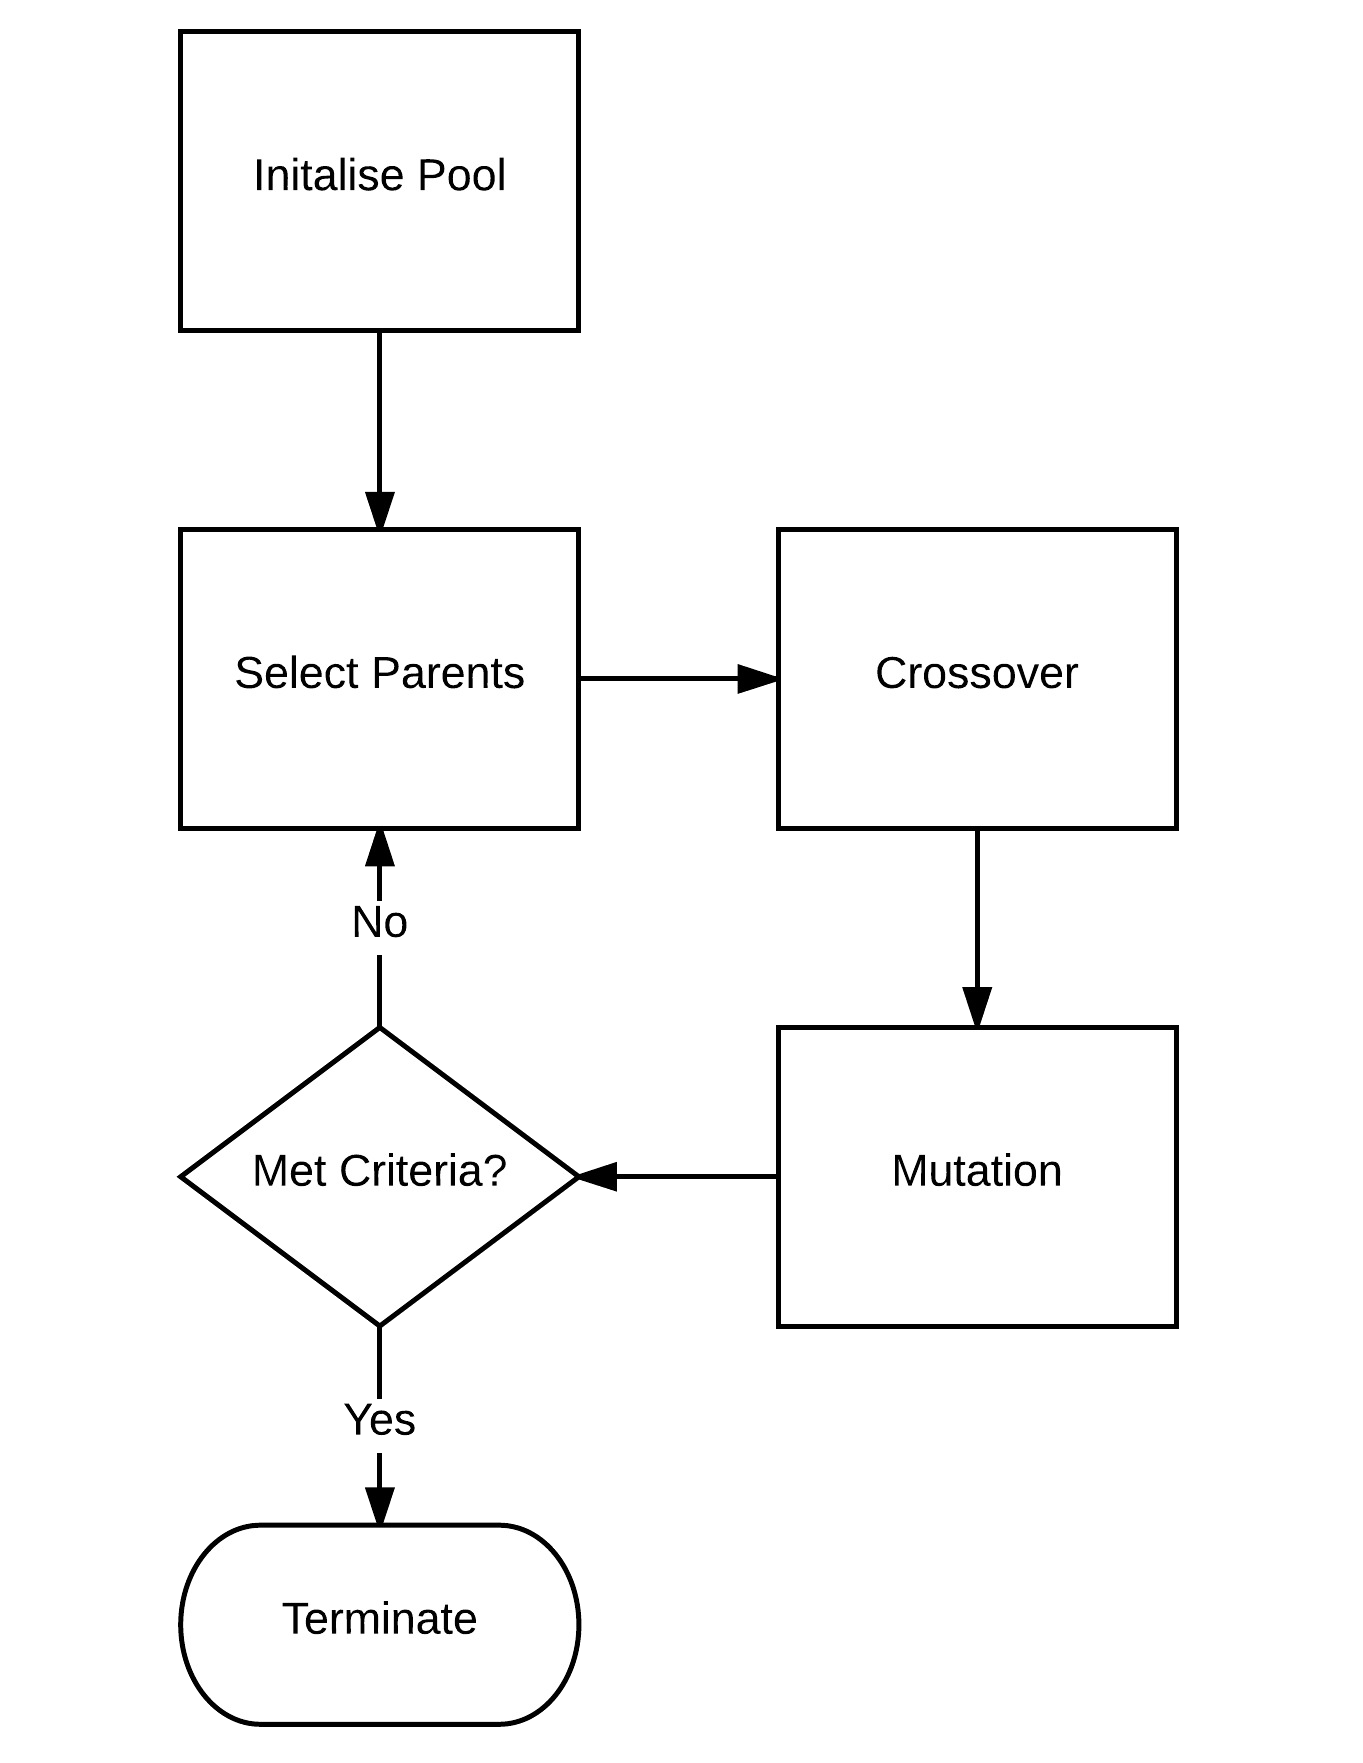
\includegraphics[width=0.5\textwidth]{GA_Structure}
	\caption{The basic structure of a Genetic Algorithm.}
	\label{struct}
\end{figure}
\noindent
A Genetic Algorithm is an algorithm that uses natural selection, or survival of the fittest, to find a solution to a problem. All Genetic Algorithms follow a similar, if not identical structure (figure \ref{struct}). However, the elements of this structure are highly customised for each specific application. Before going into detail about these elements, the concept of chromosomes and fitness must first be introduced.
\par
Chromosomes are one of the most important part of a GA, their only purpose is to store the potential solutions of the problem. How chromosomes store these solutions is up to the constructor of the GA, commonly however they are a single string that might represent a binary number, or possibly a list of the problems variables. Another important thing about chromosomes is their fitness. The fitness function of a GA describes how fit a particular problem is as a solution. How this fitness works, and how fitnesses are compared is again nearly entirely up to the constructor of the GA.


\section{Initialisation of the Pool}
\par
The first step in the execution of a Genetic algorithm is the generation of the pool. The pool is a collection of chromosomes that can be described as the "current generation". This pool is initialised by randomly generating chromosomes until the pool is filled, in the case of the research algorithm, this was done by shuffling the list of cities, thus eliminating the possibility of missing or having duplicate genes within the chromosome which was one of the constraints. The number of chromosomes in the pool is usually a fixed number, however adaptive pool sizing does exist (http://www.sciencedirect.com/science/article/pii/S2212671613000449) only fixed pool size was used in this research. 
\section{The Main Loop}
\par
This next section comprises the main body of the GA. Every time this loop is completed, a generation has passed. Through out the next sections, the methods used in the research algorithm will be used as examples.
\subsection{Parent Selection}\label{parents}
\par
Parent selection is the first step of each generation. The flow of Figure \ref{struct} suggests that all parents are selected before Crossover, however in reality it is easier and potentially more efficient to do both steps concurrently, thus you select two parents, breed them (Crossover) and repeat until a new pool is constructed.
\par
Parents can be selected in many ways, however usually the fitness of the parents is used in some way to select them. For example, in the research algorithm a method called roulette wheel selection was used (INSERT SOME REFERENCE HERE), in this method all chromosomes in the pool take up an area on a wheel proportional to the fitness of the chromosome. This created some issues as within the research algorithm as the fitness function returns the total distance of the chromosome, thus the smaller that distance the better it is. In order to get the correct probability of selection, the fitnesses needed to be 'inverted'. This was done with two equations: 
\[ inv = minFit + maxFit\]
\[ p = (inv - fitness)/totalInvFitness\]
Where $inv$ is the 'Inversion constant', $minFit$ is the smallest/best fitness in the pool, $maxFit$ is the largest/worst fitness in the pool, $p$ is the probability of selection, $fitness$ is the fitness of a chromosome, and $totalInvFitness$ is the sum of all inverted fitnesses in the pool.
\par
Using these equations, the probability of selection for each chromosome in the pool could be calculated, thus allowing for parents to be randomly selected from the pool using these probabilities.
\subsection{Crossover}\label{crossover}
\par
\begin{figure}[h]
\textit{Step 1:}
\[Parent\, 1: [0,3,\colorbox{green}{2,5,1},4]\]
\[Parent\, 2: [1,3,\colorbox{green}{5,0,4},2]\]
\[Child\, 1: [0,3,\colorbox{green}{2,5,1},4]\]
\[Child\, 2: [1,3,\colorbox{green}{5,0,4},2]\]
\textit{Step 2:}
\[Parent\, 1: [0,3,\colorbox{green}{2,5,1},4]\]
\[Parent\, 2: [1,3,\colorbox{green}{5,0,4},2]\]
\[Child\, 1: [-,3,\colorbox{green}{2,-,1},-]\]
\[Child\, 2: [-,3,\colorbox{green}{-,0,4},-]\]
\textit{Step 3:}
\[Parent\, 1: [0,3,\colorbox{green}{2,5,1},4]\]
\[Parent\, 2: [1,3,\colorbox{green}{5,0,4},2]\]
\[Child\, 1: [3,2,\colorbox{green}{-,-,-},1]\]
\[Child\, 2: [3,0,\colorbox{green}{-,-,-},4]\]
\textit{Step 4:}
\[Parent\, 1: [0,3,\colorbox{green}{2,5,1},4]\]
\[Parent\, 2: [1,3,\colorbox{green}{5,0,4},2]\]
\[Child\, 1: [3,2,\colorbox{green}{5,0,4},1]\]
\[Child\, 2: [3,0,\colorbox{green}{2,5,1},4]\]
\caption{Example of the crossover method used in the research algorithm. \label{fig:cross}}
\end{figure}
Crossover (also known as breeding) is when two chromosomes, called parents, are 'crossed' together in some way to produce one or more children. There are many ways of doing this, from slicing the parents in half and swapping the ends, to more complicated methods like the one used in the research algorithm shown in Figure \ref{fig:cross}.
\subsection{Mutation}
\par
\begin{figure}[h]
\textit{Step 1:}
\[Before: [0,3,\colorbox{green}{2},5,1,\colorbox{red}{4}]\]
\[After: [0,3,\colorbox{red}{4},5,1,\colorbox{green}{2}]\]
\caption{Example of the swap mutation used in the research algorithm \label{fig:mut}}
\end{figure}
Every child produced in Section \ref{crossover} has a chance of mutation, this is when the chromosome is subjected to a small but random change. In the case of the research algorithm, a specific form of mutation called swap mutation was used where two genes within the chromosome are randomly selected and then swapped, this is shown in Figure \ref{fig:mut}. Also, in the research algorithm, a chance of mutating multiple times was used with each subsequent mutation being less and less probable.
\section{Termination}
\par
The final step in the Genetic algorithm is termination. At the end of every generation, it is questioned whether the GA has met a specific criteria, if it has then the GA terminates and the best solution in the gene pool is the solution you finish with, otherwise it continues and begins a new generation.
\par
The criteria for termination can be nealy anything and are usually rather specific to the problem, however the are some generic ones, for example having found a solution that is better than a given solution or the simplest being having completed a given number of generations.
\section{The Research Framework}
\par
The Genetic Algorithm that was constructed for this research is divided into two components, the first being the Genetic Algorithm Framework (REFERENCE), and the second being a script which integrates with the framework.
The GAFramework is actually quite a simple program, it was designed for the research, however even though the research was specifically on the Traveling Salesman Problem, the GAF is capable of being used for any problem. It simply passes data to the scripts and provides the scripts some generic functionality such as a chromosome object and a loop function.
The script is the main bulk of the program as it is responsible for defining and solving a specific problem. The script constructed to solve the research problems was designed to be a generic script for Traveling Salesman Problems, when provided with a raw text file containing either a distance matrix or the coordinates for each city, it will proceed to solve the problem regardless of size. The script can also be given variables such as the size of chromosome pool, or the percentage of the pool to make elites. 

